\documentclass[border=10pt]{standalone}
\usepackage{tikz}
\usepackage{circuitikz}
\usetikzlibrary{positioning, calc, shapes.symbols}

% Top level of the GCD processor: control unit + datapath (block diagram).
% Block names and pin names follow gcd_control.vhd / gcd_datapath.vhd.

% pins on the left / right edge of a block:  x, y of the first pin, step, comma list of names
\newcommand{\pinsL}[4]{%
  \foreach \p [count=\i from 0] in {#4} {%
     \pgfmathsetmacro\py{#2-\i*#3}%
     \draw[thin] (#1,\py) -- ++(0.35,0);
     \node[anchor=west, label_text] at (#1+0.4,\py) {\p};
  }}
\newcommand{\pinsR}[4]{%
  \foreach \p [count=\i from 0] in {#4} {%
     \pgfmathsetmacro\py{#2-\i*#3}%
     \draw[thin] (#1,\py) -- ++(-0.35,0);
     \node[anchor=east, label_text] at (#1-0.4,\py) {\p};
  }}

\begin{document}
\makeatletter\def\pgf@circ@font@tiny{\footnotesize}\makeatother
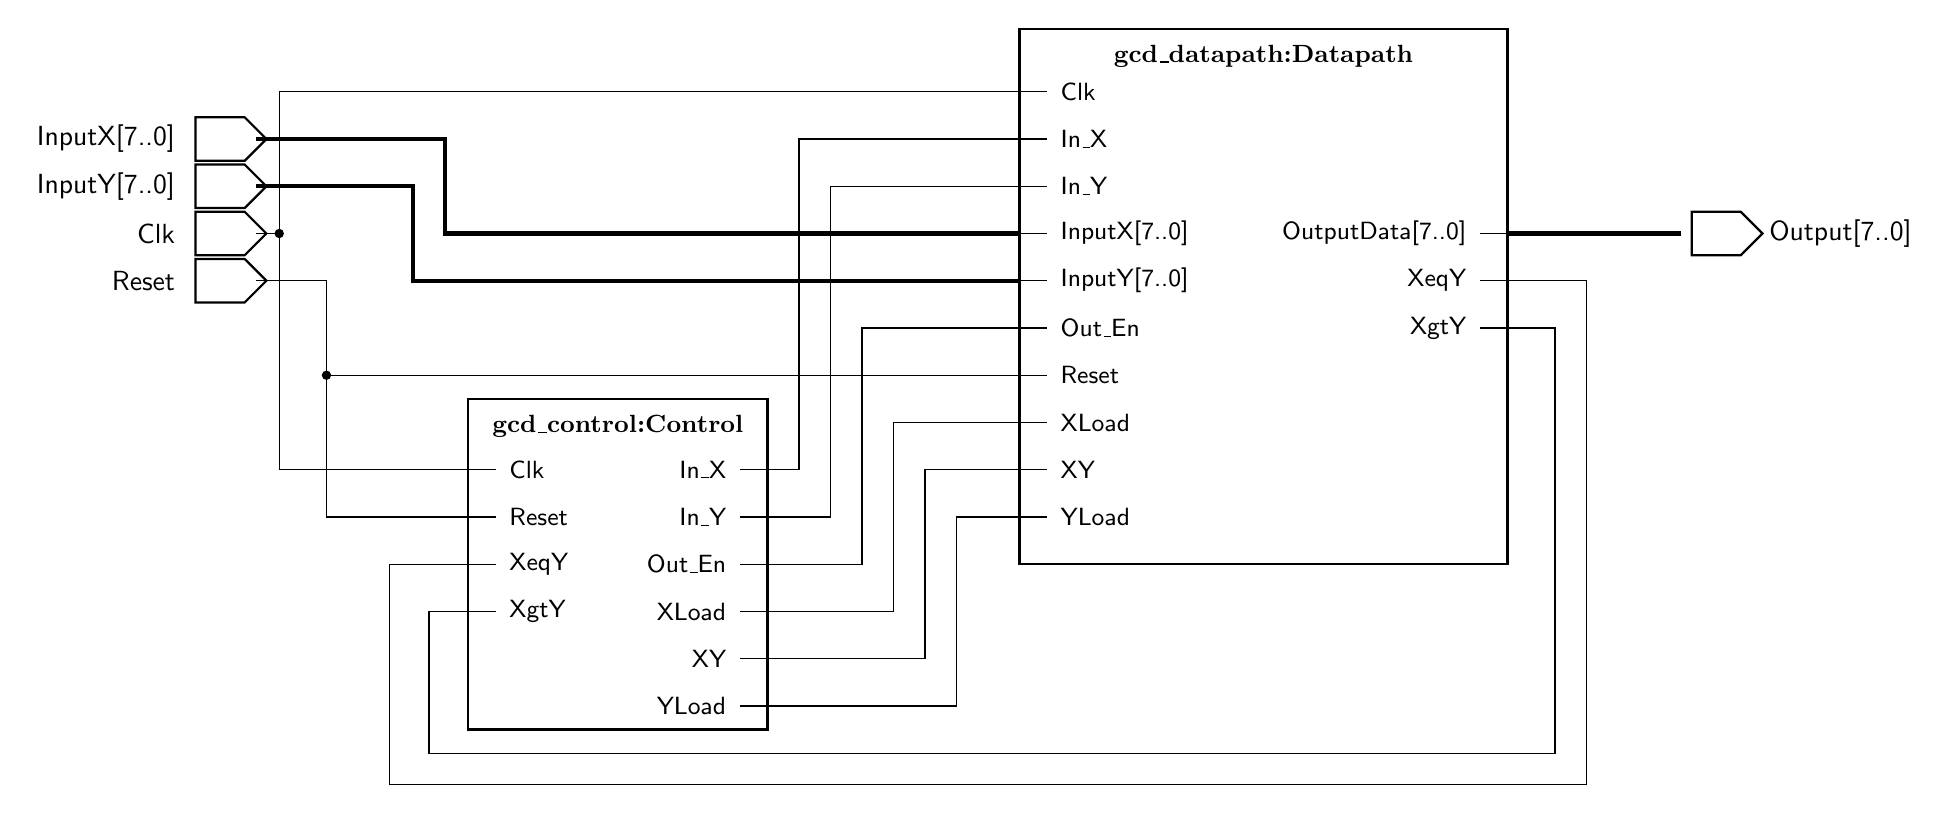
\begin{tikzpicture}[
    font=\sffamily,
    label_text/.style={font=\sffamily\small},
    wire/.style={line width=0.5pt},
    bus/.style={line width=1.5pt},
    junction/.style={circle, fill, inner sep=1.2pt},
    port/.style={signal, signal to=east, draw, thick, minimum height=0.55cm, minimum width=0.9cm, inner sep=0pt},
]

    % ---------------------------------------------------------------- blocks
    \draw[thick] (3.6,-0.9) rectangle (7.4,3.3);
    \node[font=\small\bfseries] at (5.5,2.95) {gcd\_control:Control};
    \pinsL{3.6}{2.4}{0.6}{Clk,Reset,XeqY,XgtY}
    \pinsR{7.4}{2.4}{0.6}{In\_X,In\_Y,Out\_En,XLoad,XY,YLoad}

    \draw[thick] (10.6,1.2) rectangle (16.8,8.0);
    \node[font=\small\bfseries] at (13.7,7.65) {gcd\_datapath:Datapath};
    \pinsL{10.6}{7.2}{0.6}{Clk,In\_X,In\_Y,{InputX[7..0]},{InputY[7..0]},Out\_En,Reset,XLoad,XY,YLoad}
    \pinsR{16.8}{5.4}{0.6}{{OutputData[7..0]},XeqY,XgtY}

    % ---------------------------------------------------------------- external ports
    \node[port] at (0.45,6.6) {};  \node[anchor=east] at (0,6.6) {InputX[7..0]};
    \node[port] at (0.45,6.0) {};  \node[anchor=east] at (0,6.0) {InputY[7..0]};
    \node[port] at (0.45,5.4) {};  \node[anchor=east] at (0,5.4) {Clk};
    \node[port] at (0.45,4.8) {};  \node[anchor=east] at (0,4.8) {Reset};
    \node[port] at (19.45,5.4) {}; \node[anchor=west] at (20.0,5.4) {Output[7..0]};

    % data buses
    \draw[bus] (0.9,6.6) -- (3.3,6.6) -- (3.3,5.4) -- (10.6,5.4);
    \draw[bus] (0.9,6.0) -- (2.9,6.0) -- (2.9,4.8) -- (10.6,4.8);
    \draw[bus] (16.8,5.4) -- (19.0,5.4);

    % clock and reset
    \draw[wire] (0.9,5.4) -- (1.2,5.4) -- (1.2,7.2) -- (10.6,7.2);
    \draw[wire] (1.2,5.4) -- (1.2,2.4) -- (3.6,2.4);
    \node[junction] at (1.2,5.4) {};
    \draw[wire] (0.9,4.8) -- (1.8,4.8) -- (1.8,3.6) -- (10.6,3.6);
    \draw[wire] (1.8,3.6) -- (1.8,1.8) -- (3.6,1.8);
    \node[junction] at (1.8,3.6) {};

    % control word: control unit -> datapath
    \draw[wire] (7.4,2.4)  -- (7.8,2.4)  -- (7.8,6.6) -- (10.6,6.6);
    \draw[wire] (7.4,1.8)  -- (8.2,1.8)  -- (8.2,6.0) -- (10.6,6.0);
    \draw[wire] (7.4,1.2)  -- (8.6,1.2)  -- (8.6,4.2) -- (10.6,4.2);
    \draw[wire] (7.4,0.6)  -- (9.0,0.6)  -- (9.0,3.0) -- (10.6,3.0);
    \draw[wire] (7.4,0.0)  -- (9.4,0.0)  -- (9.4,2.4) -- (10.6,2.4);
    \draw[wire] (7.4,-0.6) -- (9.8,-0.6) -- (9.8,1.8) -- (10.6,1.8);

    % status: datapath -> control unit
    \draw[wire] (16.8,4.8) -- (17.8,4.8) -- (17.8,-1.6) -- (2.6,-1.6) -- (2.6,1.2) -- (3.6,1.2);
    \draw[wire] (16.8,4.2) -- (17.4,4.2) -- (17.4,-1.2) -- (3.1,-1.2) -- (3.1,0.6) -- (3.6,0.6);

\end{tikzpicture}
\end{document}
